\documentclass{article}

\usepackage[bib,bibstyle=ieee,bibargs={sorting=none},smalltitle,code,margin=0.95in]{shorthand}
\usepackage{pgfplots,pgfplotstable}
\usepackage{subfig}

\addbibresource{Report.bib}

\def\datadir{2019-04-08-23-08-16}

\setcounter{secnumdepth}{0}

\title{Solving Differential Equations using a Forward Neural Network}
\author{Hunter Damron}
\date{9 April 2019}

\hdef{y}

\begin{document}
    \maketitle

    \section{Introduction}
        Although it originated as a mathematical model of neural activity, the forward neural network has become a popular tool in modern scientific culture. The neural network first gained popularity with Rosenblatt's perceptron~\cite{rosenblatt} and has since become widely used for function modeling with the increase in available computational power. Forward neural networks are composed of many `neurons' which are composed of a linear unit wrapped in a nonlinear function. Although the model is simple, it is capable of approximating any function, as shown by Cybenko~\cite{approx}.
    \section{Problem Statement}
        This paper presents a simple neural network to approximate the function $y = \sin(10t)$ on the range $[0,\pi/5]$ using points on the curve as training input. The resulting approximator is then generalized to the range $[0,10\pi]$.
    \section{Procedure}
        To effectively model the curve $y = \sin(10t)$, a neural network with two hidden layers, both of width 120 are used. The input $t$ and output $\hy$ are both real scalars. Each layer other than the input layer is composed of a weight matrix $W_i \in \R^{n \times m}$ and a bias $b_i \in \R^m$ where $n$ is the input dimension and $m$ is the output dimension. Every layer except the last layer is also wrapped in an activation function $f_i$ to provide nonlinearity. Combining these pieces, each layer can be formulated as \[ x_{i+1} = f(W_i x_i + b_i) \] where $x_i$ is the input to the layer and $x_{i+1}$ is the layer's output. The choice of two layers with width 120 was found experimentally to be satisfactory for the approximation.

        For training, the cost function was chosen to be the mean square error ($MSE$) of the predicted $\hy$ vs the true value $y$ \[ MSE = \frac{1}{N} \sum_{i=0}^{N-1} (\hy(t_i) - y(t_i))^2 \] where each $t_i$ is a sample point on the training range and $N$ is the number of samples. This cost function is a common choice for many machine learning applications because it is equivalent to the $L_2$-norm up to ordering but is more efficient and numerically stable because it does not take the square root. In this paper, $N = 500$ samples are used.

        A gradient descent algorithm is used for optimization with a learning rate of 0.00005. Training occured over 20000 epochs. Gradient descent was chosen because it is the simplest of the commonly used learning algorithms and has the fewest parameters.

        The TensorFlow framework~\cite{tf} was used for all numerical calculations in the project. The resulting network is shown in Figure~\ref{fig:network}

        \begin{figure}[!htbp]
            \centering
            \caption{Schematic of the network (produced using NN-SVG~\cite{schematic})} \label{fig:network}
            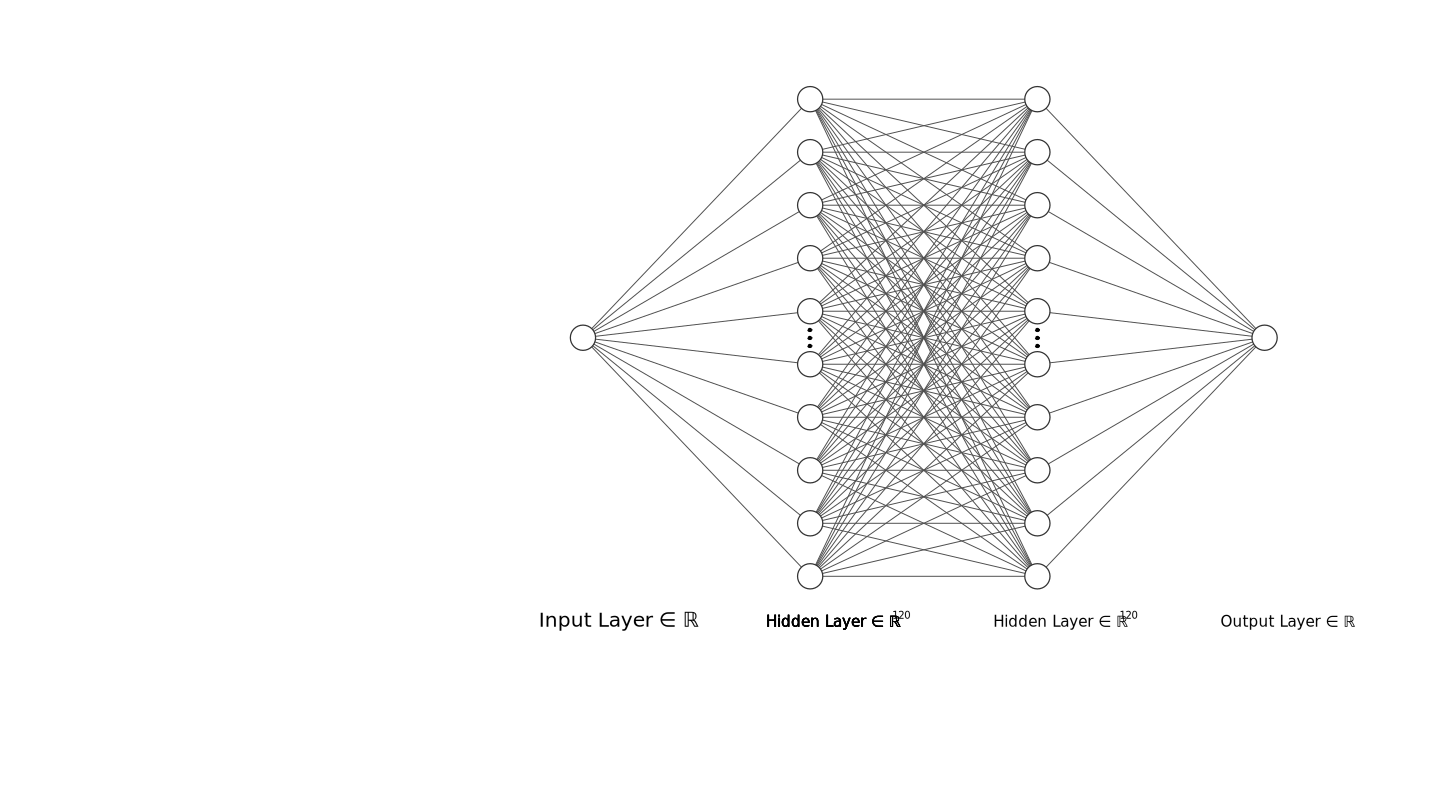
\includegraphics[width=0.6\textwidth]{nn.png}
        \end{figure}
    \section{Results}
        The results of the trained algorithm are shown in Figure~\ref{fig:output} as a comparison to the target $y=\sin(10t)$ on the training range $[0,\pi/5]$. Figure~\ref{fig:full} shows the prediction of the network when extrapolated to a much larger range $[0,10\pi]$.

        \begin{figure}[!htbp]
            \centering
            \caption{Comparison of trained approximation $\hy$ to true value of $y$ on range $[0,\pi/5]$} \label{fig:output}
            \begin{tikzpicture}
            \begin{axis}[
                    xlabel={$t$},
                    ylabel={$y$},
                    width=0.7\textwidth
                ]
                \pgfplotstableread[col sep=comma]{\datadir/Values.csv}\datavalues
                \addlegendentry{Target}
                \addplot[thick,blue,mark=none,smooth] table[y index=0, y index=1]{\datavalues};

                \addlegendentry{Experimental}
                \addplot[thick,red,mark=none,smooth] table[y index=0, y index=2]{\datavalues};
            \end{axis}
            \end{tikzpicture}
        \end{figure}

        \begin{figure}[!htbp]
            \centering
            \caption{Comparison of trained approximation $\hy$ to true value $y$ when extrapolated to range $[0,10\pi]$} \label{fig:full}
            \begin{tikzpicture}
            \begin{axis}[
                    xlabel={$t$},
                    ylabel={$y$},
                    width=0.7\textwidth
                ]
                \pgfplotstableread[col sep=comma]{\datadir/Values-full.csv}\datavaluesfull
                \addlegendentry{Target}
                \addplot[thick,blue,mark=none,smooth] table[y index=0, y index=1]{\datavaluesfull};

                \addlegendentry{Experimental}
                \addplot[thick,red,mark=none,smooth] table[y index=0, y index=2]{\datavaluesfull};
            \end{axis}
            \end{tikzpicture}
        \end{figure}

        Figure~\ref{fig:loss} shows the value of the loss function over time during training both on the training range and on the generalized range. Note that although the loss on the generalized range in Figure~\ref{fig:lossfull} decreases, it is quite large.

        \begin{figure}[!htbp]
            \centering
            \caption{Cost of $\hy$ versus $y=sin(10t)$ on training range and on generalized range}
            \subfloat[On Range {$[0,\pi/5]$}]{%
                \centering
                \begin{tikzpicture}
                \begin{axis}[
                	xlabel={Epoch},
                    ylabel={$MSE$},
                    width=0.45\textwidth
               	]
                    \addplot[thick,mark=none,smooth] table[x expr={\coordindex*100}, y index=0,col sep=comma]{\datadir/Losses-trimmed.csv};
                \end{axis}
                \end{tikzpicture}
            }
            \hfill
            \subfloat[Generalized to range {$[0,10\pi]$} \label{fig:lossfull}]{%
                \centering
                \begin{tikzpicture}
                \begin{axis}[
                    xlabel={Epoch},
                    ylabel={$MSE$},
                    width=0.45\textwidth
                ]
                    \addplot[thick,mark=none,smooth] table[x expr={\coordindex*100}, y index=1,col sep=comma]{\datadir/Losses-trimmed.csv};
                \end{axis}
                \end{tikzpicture}
            }
        \end{figure}

    \section{Discussion}
        Training on the range $[0,\pi/5]$ was achieved on the order of minutes using the described configuration and produced a decent result. With a more precise tuning of the parameters and possibly wider hidden layers, a neural network should be capable of easily approximating a single variable function on such a small range. However, when the range is extended to $[0,10\pi]$, the result is not accurate at all. After the training range, the network responds approximately linearly because there was no reason for it to change its behavior outside the training range. Although neural networks may be capable of interpolating missing data within the training range, it is impossible for them to extrapolate beyond the training range with any degree of accuracy.

        The loss function, as shown in Figure~\ref{fig:loss}, shows that the initial training happens very quickly, but the majority of training applies to the last small deviation. Attempts have been made in other optimizers to increase training speed on small deviations without sacrificing accuracy. In future exploration, these other optimization algorithms may be used. This rate of learning is also controlled by a hyperparameter which may not be optimally tuned.
    \printbibliography{}

    \appendix
    \section{Appendix}
    \setcounter{secnumdepth}{2}
    \renewcommand{\thesubsection}{\Alph{subsection}}
    \subsection{Sine Curve Neural Network} \label{apx:code1}
    \lstinputlisting{DiffEq.py}
\end{document}
